\section{Large-Scale Structure \Contact{Tony}}
\Contributors{Anthony Tyson, Rogerio Rosenfeld}
\label{sec:lss}

LSST is anticipated to produce the largest and most detailed map of the distribution of matter and the growth of cosmic structure over the past 10 billion years. The large-scale clustering of matter and luminous tracers in the late-time universe is sensitive to the total amount of dark matter, the fraction of dark matter in light relics that behave as radiation at early times, and fundamental interactions in the dark sector. For example, the high densities of matter and energy in the early universe imply that even extremely weakly coupled dark matter particles can leave detectable imprints on the galaxy distribution today. Dark matter that couples to photons, neutrinos, or a light scalar field could produce dark acoustic oscillations analogous to baryon acoustic oscillations \citep{Cyr-Racine:2014}. Large-scale structure probes would be particularly competitive for multi-component dark matter models in which only a fraction of the dark matter couples to dark radiation. Meanwhile, LSST will enable tests of dark matter with non-standard gravitational interactions, such as violations of the equivalence principle \citep{Bonvin:2018} and interactions between dark matter and dark energy. The nature of the dark matter can be broadly described by a so-called Generalized Dark Matter model \citep{Hu:1998}, which has been recently explored in a study of the dark matter equation of state through cosmic history \citep{Kopp:2018}. 
Dark matter probes involving large-scale structure highlight the interconnectedness of dark matter and dark energy research, both in terms of testing the validity of the standard cosmological paradigm, and overlap in the specific analysis methods employed. The studies described in this section are illustrative examples of how the nature of dark matter can be probed employing the same galaxy clustering and weak lensing techniques as used in dark energy constraints. 

As one specific example, measurements of large-scale structure with LSST will enhance constraints on massive neutrinos and other light relics from the early universe that could compose a fraction of the dark matter. The combination of galaxy imaging and redshift surveys together with CMB experiments in the coming decade will make it possible to measure the density of relativistic particles in the early Universe at the percent level. The existence of the cosmic neutrino background can already be inferred from temperature fluctuations of the CMB \citep{Planck:2018_cosmo_params} and Big Bang nucleosynthesis \citep{Cooke:2018}, and a major goal of upcoming cosmology experiments is to measure the sum of neutrino masses at the few milli-eV level using weak gravitational lensing and galaxy clustering \citep[e.g.,][]{CMB-S4:2016,DESI:2016,Mishra-Sharma:2018}.\footnote{The LSST Dark Energy Science Collaboration ``Science Roadmap'' is available at \url{http://lsstdesc.org/sites/default/files/DESC_SRM_V1_4.pdf}} In the standard cosmological model with three neutrinos, the effective number of relativistic free-streaming species is $N_{\rm eff}$ = 3.046. Several classes of dark matter models, such as axions, axion-like particles, dark photons, and light sterile neutrinos, predict deviations in $N_{\rm eff}$ that could be measurable with LSST and CMB experiments, even if the light species decouple before the QCD phase transition \citep{Font-Ribera:2014,Baumann:2018}. Galaxy surveys contribute to constraints on $N_{\rm eff}$ by independently constraining the Hubble constant, which is partially degenerate with $N_{\rm eff}$, and importantly, by measuring the broadband shape and phase of the galaxy power spectrum, which are sensitive to the gravitational influence of free-streaming light relics. The broadband galaxy power spectrum can also add robustness to the CMB results on $N_{\rm eff}$ because it is less dependent on the primordial helium abundance.

\begin{figure}[t]
\centering
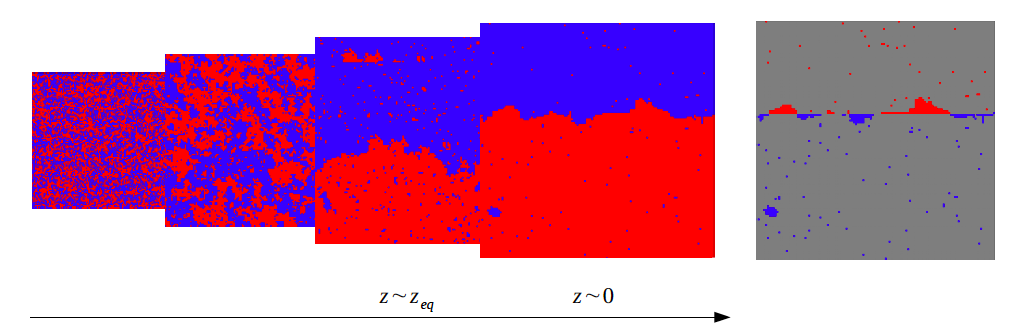
\includegraphics[width=0.9\columnwidth]{DMDE-anisotropy.png}
\caption{A schematic diagram of the emergence of dark energy anisotropy from an Ising model phase transition and a coupling with the anisotropic distribution of dark matter. Figure taken from \citet{1810.11007}.}
\label{fig:DMDEmap}
\end{figure}

Another example demonstrating the potential of large-scale structure to study dark matter involves probing a possible coupling to dark energy, e.g., if dark energy were an aspect of dark matter at late times.
%The physics of dark matter could be probed via LSST 
The natural inhomogeneities in dark matter on large scales would then be reflected as spatial inhomogeneities in the developing late-time acceleration. 
This could be observed as spatial variations in cosmic acceleration by LSST correlated with the large scale dark matter weak lensing maps. 
Such a spatial correlation is a generic prediction if dark matter and dark energy are causally related or if dark energy is emergent \citep{1801.09658}. 
A spatially complicated potential leads to a small cosmological constant from an energy difference between its global and local minima, and dark energy and dark matter are thereby intertwined. 
If so, and if the universe on sub-horizon scales is not homogeneous, then spatial fluctuations in one component should be correlated with spatial fluctuations in the other, particularly near the epoch of emergence.

There are other models where dark matter and dark energy are intertwined, such as models where they interact 
\citep{Amendola:1999er,Holden:1999hm}.
Interacting models can be described phenomenologically via two fluids that can exchange energy and momentum, 
described by energy-momentum tensors that are not individually conserved. One can parameterize the coupling of
dark matter and dark energy by writing the divergence of the individual energy-momentum tensors as 
\begin{eqnarray}
\nabla_{\mu} T^{(DE)}\,^{\mu}_{\nu} &=& C^{(DE)}_{\nu}, \label{cons_phi} \\
\nabla_{\mu} T^{(DM)}\,^{\mu}_{\nu} &=& C^{(DM)}_{\nu}, \label{cons_dm}
\end{eqnarray}
where the superscript $(DM)$ stands for the dark matter fluid and $(DE)$ for the dark energy.
The conservation of the total dark component energy-momentum tensor 
(we assume the separate conservation of the energy momentum of radiation and baryons),
\begin{equation}
\label{energyconservation}
\nabla_{\mu} \left[ T^{(DM)} \,^{\mu}_{\nu} + T^{(DE)} \,^{\mu}_{\nu} \right]= 0,
\end{equation}
implies that
\begin{equation}
C^{(DM)}_{\nu}=-C^{(DE)}_{\nu}.
\end{equation}

The coupling between dark matter and dark energy is determined by the function $C^{(DM)}_{\nu}$ which is usually
written as
\begin{equation}
C^{(DM)}_{\nu} = (8\pi G)^{1/2} \,\beta\rho_{DM}\nabla_{\nu} \phi,
\end{equation}
where $\beta$ is a constant that expresses the coupling strength. In this model, dark energy must be dynamical and here it is modeled by a scalar field  $\phi$, such as a quintessence field.
In this model, $\beta$ is the only new parameter in addition to the usual description of the dark energy sector.
The standard uncoupled case is recovered for $\beta=0$.

There is a vast literature studying this class of models that can modify both the evolution of the 
background cosmology as well as the evolution of perturbations. For instance, it has been recently claimed
that such a model can ease the tension in the measurements of $\sigma_8$ from CMB and galaxy surveys 
\citep{Barros:2018efl}.

LSST can separately map dark matter and dark energy at a redshift where they have roughly comparable influences on the expansion rate of the universe. 
There are two complementary methods of reconstructing dark energy on the sky: SNe and 3$\times$2pt in 20 degree patches \citep[Figure 15.9 in ][]{0912.0201}.
The transition between a dark matter-dominated universe to one with late-time acceleration (dark energy) may hint at some connection between these two components. 
An angular cross correlation between maps of dark energy and tomographic weak lens maps of dark matter could yield a non-zero signal.  
If so, the ratio of the cross correlation to the auto-correlations would be a diagnostic of the underlying physics. 
In this scenario, measurements of dark energy anisotropy become a probe of the nature of dark matter; \figref{DMDEmap}, reproduced from \cite{1810.11007}, illustrates a Ginzburg-Landau phase transition model that results in correlated dark matter-dark energy anisotropy. 
Quadrupole and higher-order correlated anisotropies are generated around redshift $z=0.7$.  
This is accessible in LSST maps of dark energy and dark matter in a broad redshift shell.

\paragraph{Systematics and synergies:}
Systematics in the dark energy and dark matter maps on large angular scales must be reduced below the level of any dark matter-dark energy correlation signal.  
For example, systematics in apparent magnitude and \photoz due to uncorrected extinction from Galactic dust would be one focus. 
Encouragingly, the two measures of dark energy anisotropy depend differently on wavelength-dependent extinction. 
A useful null test will be the cross correlation between dark energy and dark matter maps with dust maps.  
This would set the floor for residual extinction systematics, forming the basis for a forward simulation of the resulting dark energy-dark matter false correlation. 
As in analysis of CMB data, cuts on Galactic latitude can reveal the level of residual systematics. 
Finally, any dependence of the cross-correlations on redshift could discriminate between models as well as detect redshift-dependent systematics.

For detection of low multipole sky correlations, observations in the north as well as the south will be useful.
There is important synergy with WFIRST and EUCLID observations in the north.  
These complementary data could be calibrated and tested by joint null tests in overlap areas with the LSST survey.